\section{Theorie}
\label{sec:Theorie}

Mithilfe der Röntgenreflektometrie sollen Dichte, Rauigkeit und Schichtdicke eines Polystyrolfilms bestimmt werden.

\subsection{Grundlagen}

Brechung findet statt, wenn eine elektromagnetische Welle von einem Medium mit Brechungsindex $n_1$ in ein anderes Medium mit 
Brechungsindex $n_2$ eintritt. Dabei muss gelten, dass $n_1 \neq n_2$. In diesem Versuch wird Röntgenstrahlung mit einer 
Wellenlänge $\lambda$ im Bereich $\SI{0.1}{\angstrom}-\SI{10}{\angstrom}$ betrachtet. \\
Für den Brechungsindex gilt 

\begin{equation*}
    n = 1-\delta +i\beta,
\end{equation*}

wobei $\delta$ ein Korrekturterm und $\beta$ die Absorption ist. Für Röntgenstrahlung gilt, dass der Brechungsindex kleiner als 
eins ist. \\
Mit dem Snelliusschen Berechungsgesetz

\begin{equation*}
    \frac{n_1}{n_2} = \frac{\cos{\left(\alpha_2\right)}}{\cos{\left(\alpha_1\right)}}
\end{equation*}

und der Annahme, dass die Grenzfläche der Medien eine homogene Ebene ist, ergibt sich ein kritischer Winkel $\alpha_\text{C}$, 
bei dem eine Totalreflexion auftritt. Unter Vernachlässigung der Absorption folgt für kleine Winkel nährungsweise

\begin{equation*}
    \alpha_\text{C} \approx \sqrt{2\delta} = \lambda \sqrt{\frac{r_\text{e}\rho}{\pi}}.
\end{equation*}

Dabei ist $r_\text{e}$ der klassische Elektronenradius und $\rho$ die Elektronendichte des betrachteten Materials. 

\subsection{Fresnelsche Formeln}

Bei der Betrachtung von Reflexion und Transmission elektromagnetischer Wellen muss im Allgemeinen die Polarisation dieser 
berücksichtigt werden. Dies tun die Fresnelschen Formeln. Für s-Polarisation des Lichtes ergeben sich die Koeffizienten zu 

\begin{align*}
    r &= \frac{n_1 \cos{\left(\alpha_1\right)}-n_2 \cos{\left(\alpha_2\right)}}{n_1 \cos{\left(\alpha_1\right)}+n_2 \cos{\left(\alpha_2\right)}},\\
    t &= \frac{2n_1}{n_1 \cos{\left(\alpha_1\right)}+n_2 \cos{\left(\alpha_2\right)}}.
\end{align*}

Dabei ist hier eine Unterscheidung zwischen $p$- und $s$-Polarisation nicht notwendig, weil $n_1 \approx n_2$ gilt.\\
Die Fresnelreflektivität für Röntgenstrahlung ist für $\alpha_i > 3\alpha_\text{C}$ nährungsweise gegeben als

\begin{equation*}
    R_\text{F} = |r^2| = \left(\frac{a_\text{C}}{2\alpha_i}\right)^4.
\end{equation*}

\subsection{Mehrschichtsysteme}

In diesem Versuch wird ein Polystyrolfilm auf einem Siliziumsubstrat betrachtet, weswegen der Umgang mit Mehrschichtsystemen 
erläutert werden muss. Ein Beispiel für die Reflektivität eines solchen Systems ist in Abbildung \ref{fig:mss} zu sehen. 

\begin{figure}
  \centering
  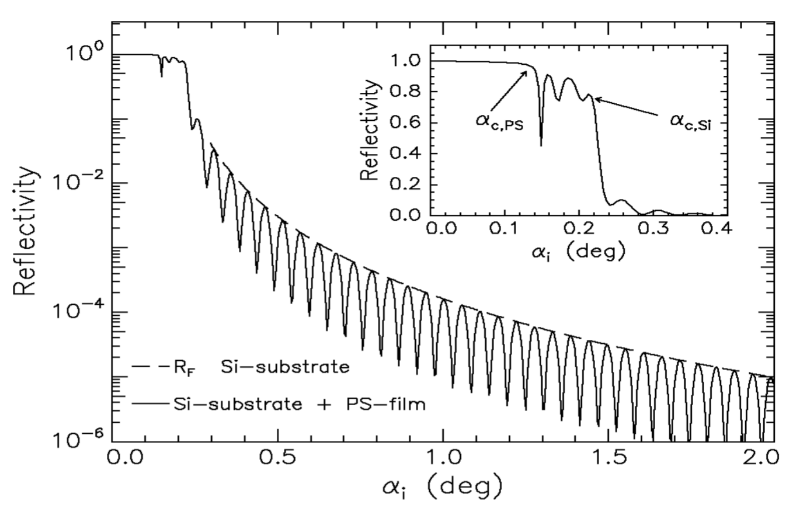
\includegraphics[scale=0.4]{content/mehrschichtsys.png}
  \caption{Beispielhafte Reflektivität eines Mehrschichtsystems aufgetragen gegen den Einfallswinkel $\alpha_i$.\cite{Anleitungalt}}
  \label{fig:mss}
\end{figure}

Dabei sind in dem vergrößerten Ausschnitt zwei Totalreflexionen zu erkennen. Diese sind dem Siliziumsubstrat und dem Polystyrolfilm
zuzuordnen. Die beobachteten Oszillationen beim Abfall der Reflektivität treten aufgrund von Interferenzeffekten an der Oberfläche 
auf. Durch diese Oszillationen sind demnach Rückschlüsse auf den Schichtabstand möglich, da bei einer destruktiven Intereferenz 
ein Gangunterschied von einem ungeraden Vielfachen von $\frac{\lambda}{2}$ vorliegen muss. Damit folgt der Zusammenhang

\begin{equation*}
    d = \frac{2\pi}{\delta q_z} = \frac{\lambda}{2\delta\alpha_1},
\end{equation*}

wobei $\vec{q} = \vec{k_2}-\vec{k_1}$ und $q_2 = 2k\sin{\left(\alpha_1\right)}$ gilt.\\

Wenn das betrachtete System $N+1$ Schichten hat, kann die Reflektivität mithilfe des rekursiven Parratt-Algorithmuses 
berechnet werden. Ein solches System ist in Abbildung \ref{fig:ns} dargstellt. 

\begin{figure}
    \centering
    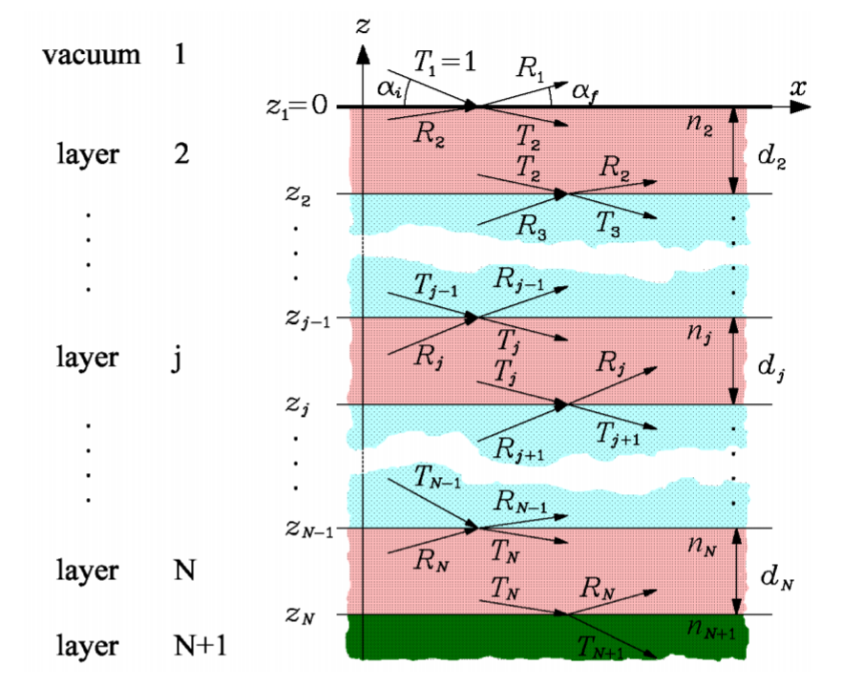
\includegraphics[scale=0.3]{content/nschichten.png}
    \caption{Beispielhafte Darstellung eines Mehrschichtsystems mit $N+1$ Schichten.\cite{Anleitungalt}}
    \label{fig:ns}
  \end{figure}

Bei dem Parratt-Algorithmus wird die Annahme getroffen, dass die unterste Schicht unendlich dick ist. An dieser
kann demnach keine Transmission stattfinden. Mathematisch wird der Algorithmus beschrieben durch 

\begin{equation*}
    X_j = \frac{R_j}{T_j} = \exp{\left(-2ik_{z,j}z_j\right)}\cdot \frac{r_{j,j+1}+X_{j+1}\exp{\left(2ik_{z,j+1}z_j\right)}}{1+r_{j,j+1}X_{j+1}\exp{\left(2ik_{z,j+1}z_j\right)}}.
\end{equation*}

Dabei beschreibt $r_{j,j+1}$ die Fresnelreflektivität an der $j$-ten Grenzfläche.\\
Mit der Startbedingung, dass an der untersten Schicht keine Reflexion stattfindet $R_{N+1} = 0$, können die Verhältnisse der
reflektierten und transmittierten Anteile rekursiv von unten nach oben berechnet werden.

\subsection{Rauigkeit}

Bisher wurde angenommen, dass die Oberfläche der Grenzfläche perfekt glatt ist. Dies ist in der Realtität nicht der Fall, 
weswegen diese Unperfektion in der Berechnung der Reflektivität berücksichtigt werden muss. Dies geschieht über eine 
Modifikation der Fresnelkoeffizienten:

\begin{align*}
    \tilde{r}_{j,j+1} &= r_{j,j+1} \exp{\left(-2k_{z,j}k_{z,j+1}\sigma_j^2\right)},\\
    \tilde{t}_{j,j+1} &= t_{j,j+1} \exp{\left(\left(k_{z,j-k_{z,j+1}}\right)^2\cdot\frac{\sigma_j^2}{2}\right)}.
\end{align*}

\subsection{Geometriefaktor und Geometriewinkel}

In Abbildung \ref{fig:geo} ist zu sehen, dass der verwendete Strahl eine größere Fläche überstreicht als die Probenoberfläche. 

\begin{figure}
  \centering
  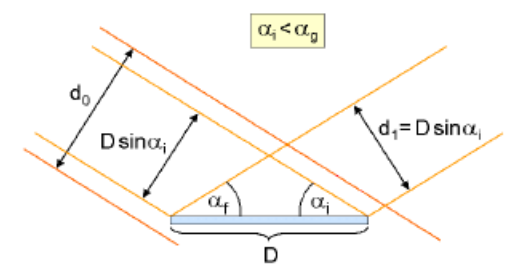
\includegraphics[scale=0.5]{content/geo.png}
  \caption{Veranschaulichung des Geometriewinkels.\cite{Anleitung}}
  \label{fig:geo}
\end{figure} 


Aus diesem Grund kann nur ein Teil der Intensität $I$ reflektiert und später detektiert werden. Dies wird durch den 
Geometriefaktor $G$ berücksichtigt:

\begin{align}
    \label{eqn:geome}
    G &= \frac{D\sin{\left(\alpha_i\right)}}{d_0} \qquad &\text{mit} \qquad \alpha_i < \alpha_g,\\
    G &= 1 \qquad &\text{mit} \qquad \alpha_i > \alpha_g.
\end{align}

Dabei ist $D\sin{\left(\alpha_i\right)}$ die Strahlbreite, die die Probenoberfläche trifft und $d_0$ die gesamte
Strahlbreite.  